\chapter{Motivaci\'on y estrategia}
\label{ch:motRadio}

\textbf{Decir algo del tamanho dle frente de onda y la frecuencia de la radiacion.}

Si bien la emisi\'on de radio de las EAS fue observada por primera vez por Jelley en 1964 \cite{jelley1966radio} y su investigaci\'on fue bastante activa durante los a\~nos 70 \cite{allan1971progress}, no fue sino hasta las \'ultimas d\'ecadas que desarrollos en electr\'onica de alta velocidad y en teor\'ia de la informaci\'on renovaron el inter\'es en el \'area.
Como consecuencia de este resurgimiento se han impulsado varios experimentos que buscan estudiar el potencial de la t\'ecnica, como por ejemplo CODALEMA \cite{ardouin2005radio}, LOPES \cite{huege2012lopes}, LOFAR \cite{horandel2009lofar}, Tunka-Rex \cite{schroder2013tunka} o AERA \cite{kelley2011aera}, la extensi\'on de radio del observatorio Pierre Auger.
Asimismo esto produjo la necesidad de desarrollar nuevas t\'ecnicas de calculo anal\'iticas \cite{huege2003radio,scholten2008macroscopic}, m\'etodos de Monte Carlo \cite{huege2007monte,ludwig2011reas3} o m\'etodos semi-anal\'iticos\cite{scholten2009macroscopic}.

El interés en la técnica reside en que la amplitud del pulso de radio generado en las antenas se encuentra correlacionado con el número de partículas y la energía de la cascada electromagnética, lo que provee información calorimétrica sobre el primario, de manera similar a la técnica de fluorescencia.
Adem\'as, los pulsos almacenados por un arreglo de antenas guardan información sobre el desarrollo longitudinal de la cascada y su $X_{max}$, es decir, son sensibles a la composici\'on de los rayos c\'osmicos primarios \cite{cite:hauge_rec,cite:lofar_rec}.
Finalmente, los arreglos de antenas de radio comparten con los de detectores de partículas sus dos principales ventajas, la reconstrucción de la dirección de arribo se realiza a partir de la medición de tiempos de disparo y su ciclo de trabajo es cercano al \cant{100}{\%}\footnote{por ejemplo, los períodos en los que haya tormentas eléctricas deben descartarse.}.
Todas estas características, sumadas al bajo costo que posee cada antena respecto a los detectores convencionales de partículas hacen de esta técnica de detección una opción competitiva para la próxima generación de detectores de rayos c\'osmicos ultra energ\'eticos.

La segunda parte de esta tesis corresponde al estudio de las capacidades y limitaciones de un arreglo de superficie de 90000 antenas de radio, desplegadas sobre una superficie de al rededor de \cant{\sim60000}{km^2}, a la hora de detectar neutrinos cósmicos ultra energéticos.
Estos números surgen de que la siguiente generación de detectores de superficie requerir\'a aumentar el área cubierta y la cantidad de estaciones respecto del de Auger (que posee el detector de superficie de punta), y al mismo tiempo, mantener la granularidad (distancia entre detectores) con el fin de conservar el nivel de eficiencia a baja energ\'ia (\cant{\sim 10^{17}}{eV}).
Actualmente existe un proyecto llamado Giant Radio Array for Neutrino Detection (GRAND)~\cite{cite:grand_prop}, que planea la instalaci\'on de 90000 antenas en un arreglo cuadrado de \cant{800}{m} de paso sobre una superficie de \cant{60000}{km^2} en la cordillera de Tianshan \cite{cite:grand_tec} con el fin de detectar neutrinos c\'osmicos ultra energ\'eticos.

Con el fin de calcular el desempe\~no del detector en esta parte del trabajo se utiliz\'o una estrategia similar a la desarrollada en Auger, ya descripta en el cap\'itulo \ref{ch:estrategiaAuger}, pero con algunas diferencias. Esta se esquematiza en la figura \ref{fig:analysisSchemaRadio}.
%
\begin{figure}[h!]
	\begin{center}
		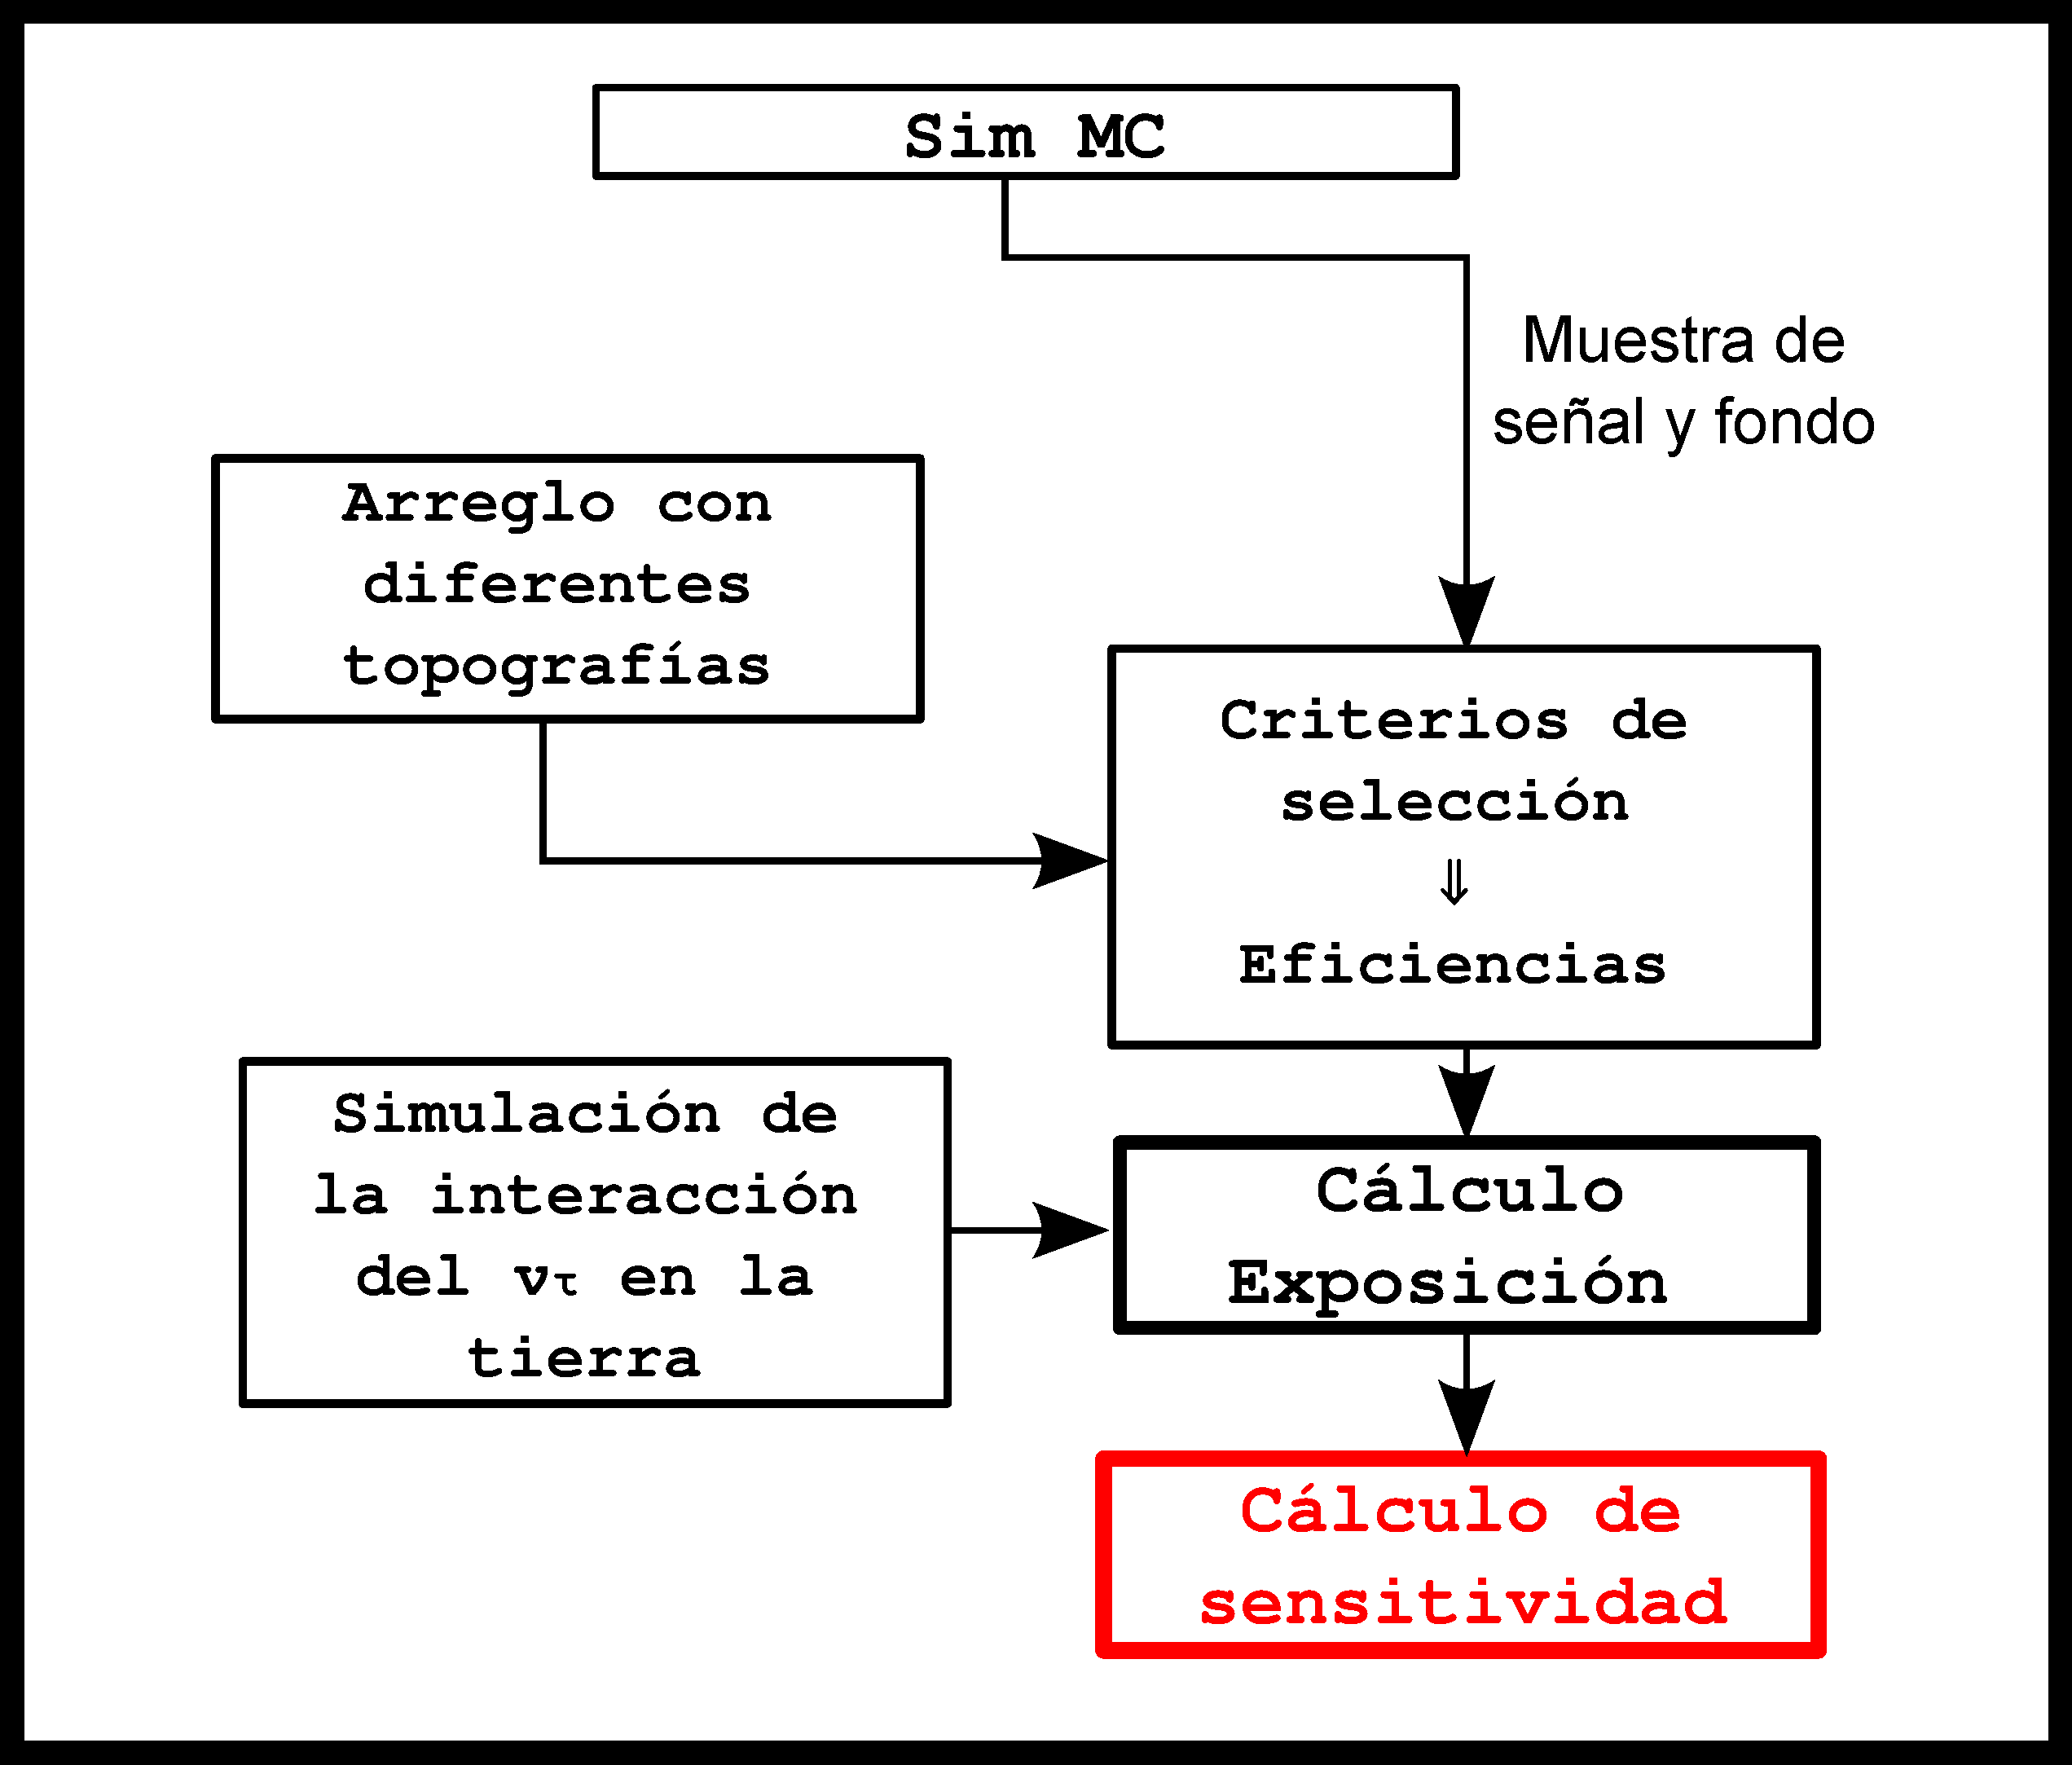
\includegraphics[width=0.9\textwidth]{fig/motivacionRadio/analysisSchemaRadio}
		\caption{Esquema de la estrategia utilizada para calcular la sensitividad del arreglo de antenas. Se utiliz\'o simulaciones de Monte Carlo de la se\~nal y del fondo para idear criterios de selcci\'on sencillos y para determinar las eficiencias de disparo e identificaci\'on. A su vez, el c\'alculo de eficiencias se realiz\'o sobre un arreglo de antenas de topograf\'ia variable. Luego, el c\'alculo de la exposici\'on se realiz\'o siguiendo la misma idea que en el an\'alisis realizado para Auger. Por \'ultimo, como medida del desempe\~no del detector se opt\'o por la sensitividad.}
		\label{fig:analysisSchemaRadio}
	\end{center}
\end{figure}
%
Las diferencias de este an\'alisis respecto del realizado para Auger provienen principalmente de que, al no existir el detector, es necesario realizar muchos supuestos como por ejemplo su topograf\'ia, las cualidades de las antenas, la ubicaci\'on geogr\'afica, entre otros.
Por otro lado, al no contar con una muestra de datos como muestra de fondo, fue necesario recurrir a simulaciones Monte Carlo de eventos hadr\'onicos inclinados.

La organizaci\'on de esta segunda parte de la tesis es la siguiente.
En el capítulo \ref{ch:easRadio} se realiza una introducción a la emisión de radio de las lluvias atmosféricas en la que se discutirán sus características principales, sus mecanismos de producción y se discutirá un modelo simplificado que mediante hipotesis geom\'etricas permite recuperar sus características principales.
Más adelante, el capítulo \ref{ch:simulacionRadio} se dedica a describir la cadena de simulaciones utilizadas para el c\'alculo de la se\~nal en el detector. 
En particular, contiene una revisión detallada de \zhs{}, el programa utilizado para simular la emisión de radio de las EAS y una caracterización de las señales a nivel del suelo que generan los neutrinos ES junto a posibles estrategias para separar eventos generados por neutrinos ES de los producidos por lluvias protonicas horizontales.
Finalmente en el capítulo \ref{ch:resultadosRadio} se calculan las eficiencias de disparo e identificaci\'on, la exposición y la sensitividad que podría alcanzar un detector de superficie de 90000 antenas de radio, considerando diferentes topografías.

\textbf{XXX HACER UN RECUENTO DE LO QUE HAY EN LA SEGUNDA PARTE DE LA TESIS}

